\documentclass{beamer}

% Thematics
\PassOptionsToPackage{subsection=false}{beamerouterthememiniframes}
\usetheme{Szeged}
\usecolortheme{beaver}
\setbeamercolor{block title}{fg=darkred}
\setbeamercolor{item}{fg=darkred}
\setbeamertemplate{navigation symbols}{}
\let\oldsection\section
\renewcommand{\section}[1]{\oldsection{\textsc{#1}}\subsection{}}

% Graphics
\usepackage{graphicx}
\usepackage[pdf]{pstricks}
\psset{unit=0.9in,linewidth=0.02,arrows=C-C,arrowsize=0.2}
\newcommand{\pscophylogeny}{
\begin{pspicture}(18,12)
\psset{unit=0.2cm,linewidth=0.2,arrowsize=0.2}
\psline[linecolor=blue](0,0)(10,10)
\psline[linecolor=blue](4,0)(2,2)
\psline[linecolor=blue](8,0)(4,4)
\psline[linecolor=blue](12,0)(14,2)
\psline[linecolor=blue](16,0)(8,8)
\psline[linecolor=red](1,0)(11,10)
\psline[linecolor=red,arrows=-o](17,0)(9,8)
\psline[linecolor=red,arrows=-o](13,0)(15,2)
\psline[linecolor=red](7,3)(14,3)
\psline[linecolor=red,arrows=<-](10,3)(14,3)
\psline[linecolor=red](10,0)(7,3)
\psline[linecolor=red,arrows=-o](9,0)(5,4)
\psline[linecolor=red,arrows=-o](4,1)(3,2)
\rput{135}(4,1){\LARGE\textcolor{red}{\textsf{\textbf{x}}}}
\psline[linecolor=red](18,0)(17,1)
\psline[linecolor=red,arrows=*-](16,1)(17,1)
\end{pspicture}
}

% Maths
\usepackage{amsmath}
\usepackage{mathtools}
\usepackage{commath}
\newcommand{\R}{\ensuremath{\mathcal{R}}}

% Puzzle

\usepackage{tikz}
\usetikzlibrary{calc}
\usetikzlibrary{scopes}

\makeatletter

\newif\ifpuzzle@hole
\newif\ifpuzzle@hole@A
\newif\ifpuzzle@hole@B
\newif\ifpuzzle@hole@C
\newif\ifpuzzle@hole@D
\def\puzzle@width{0.25cm}
\def\puzzle@height{0.20cm}
\def\puzzle@holes{true,true,false,false}
\def\puzzle@set@hole@A#1,#2,#3,#4,{\csname puzzle@hole@A#1\endcsname}
\def\puzzle@set@hole@B#1,#2,#3,#4,{\csname puzzle@hole@B#2\endcsname}
\def\puzzle@set@hole@C#1,#2,#3,#4,{\csname puzzle@hole@C#3\endcsname}
\def\puzzle@set@hole@D#1,#2,#3,#4,{\csname puzzle@hole@D#4\endcsname}
\pgfkeys{/puzzle/width/.store in=\puzzle@width}                      
\pgfkeys{/puzzle/height/.store in=\puzzle@height}                    
\pgfkeys{/puzzle/holes/.store in=\puzzle@holes}                      
                                                                        

\def\drawPuzzleSide#1#2#3{%
    let \p{mid}=($(#1)!0.5!(#2)$),
        \p{diff}=($(#2)-(#1)$),   
        \p{diff 90}=($(0,0)!1.0!\csname ifpuzzle@hole@#3\endcsname90\else270\fi:(\p{diff})$),                                                                   
        \n{len}={veclen(\x{diff},\y{diff})},                                    
        \n{height}={\puzzle@height},                                            
        \n{width}={\puzzle@width},                                              
        \p{dy}=($(\n{height}*\x{diff 90}/\n{len},\n{height}*\y{diff 90}/\n{len})$),                                                                             
        \p{dx}=($(\n{width}*\x{diff}/\n{len},\n{width}*\y{diff}/\n{len})$),     
        \p{xx}=($(\p{diff})-(\p{dx})$),                                         
        \p{11}=($(#1)+0.20*(\p{xx})-0.020*(\p{diff 90})$),                      
        \p{12}=($(#1)+0.35*(\p{xx})-0.030*(\p{diff 90})$),                      
        \p{13}=($(\p{mid})-0.5*(\p{dx})-0.030*(\p{diff 90})$),                  
        \p{21}=($(#2)-0.20*(\p{xx})-0.020*(\p{diff 90})$),                      
        \p{22}=($(#2)-0.35*(\p{xx})-0.030*(\p{diff 90})$),                      
        \p{23}=($(\p{mid})+0.5*(\p{dx})-0.030*(\p{diff 90})$),                  
        \p{14}=($(\p{13})+0.60*(\p{dx})+0.80*(\p{dy})$),                        
        \p{24}=($(\p{23})-0.60*(\p{dx})+0.80*(\p{dy})$),                        
        \p{00}=($(\p{mid})+(\p{dy})$),                                          
        \p{15}=($(\p{00})-1.6*(\p{dx})-0.04*(\p{dy})$),                         
        \p{25}=($(\p{15})!2.0!(\p{00})$)                                        
    in .. controls (\p{11}) and (\p{12}) .. (\p{13})                            
       .. controls (\p{14}) and (\p{15}) .. (\p{00})                            
       .. controls (\p{25}) and (\p{24}) .. (\p{23})                            
       .. controls (\p{22}) and (\p{21}) .. (#2)                                
}                                                                               

\def\puzzle@set@holes{%
    \expandafter\puzzle@set@hole@A\puzzle@holes,
    \expandafter\puzzle@set@hole@B\puzzle@holes,
    \expandafter\puzzle@set@hole@C\puzzle@holes,
    \expandafter\puzzle@set@hole@D\puzzle@holes,
}
\def\drawPuzzlePiece{%
   let \p1=(\tikztostart),
       \p2=(\tikztotarget) in
    (\p1) \drawPuzzleSide{\p1}{\p1-|\p2}{A}
          \drawPuzzleSide{\p1-|\p2}{\p2}{B}
          \drawPuzzleSide{\p2}{\p1|-\p2}{C}
          \drawPuzzleSide{\p1|-\p2}{\p1}{D}
}

\tikzset{test/.style={to path={\drawPuzzlePiece}}}
\tikzset{puzzle piece/.style={to path={\drawPuzzlePiece},
                              execute at begin to=\puzzle@set@holes}}

\makeatother

\usepackage{hanging}

\newcommand\blfootnote[1]{
  \begingroup
  \renewcommand\thefootnote{}\footnote{#1}
  \addtocounter{footnote}{-1}
  \endgroup
}

% Title page
\title[Bayesian Reconstruction of Coevolutionary Histories]{Bayesian Reconstruction of \\ Coevolutionary Histories}
\author{Arman Bilge}
\institute[Arman Bilge]{\vspace{-0.25in}\\Faculty of Science\\The University of Auckland}
\date{\vspace{-0.25in}\\December 9, 2013}
\titlegraphic{
%\vspace{-1in}
%\mbox{}
%\llap{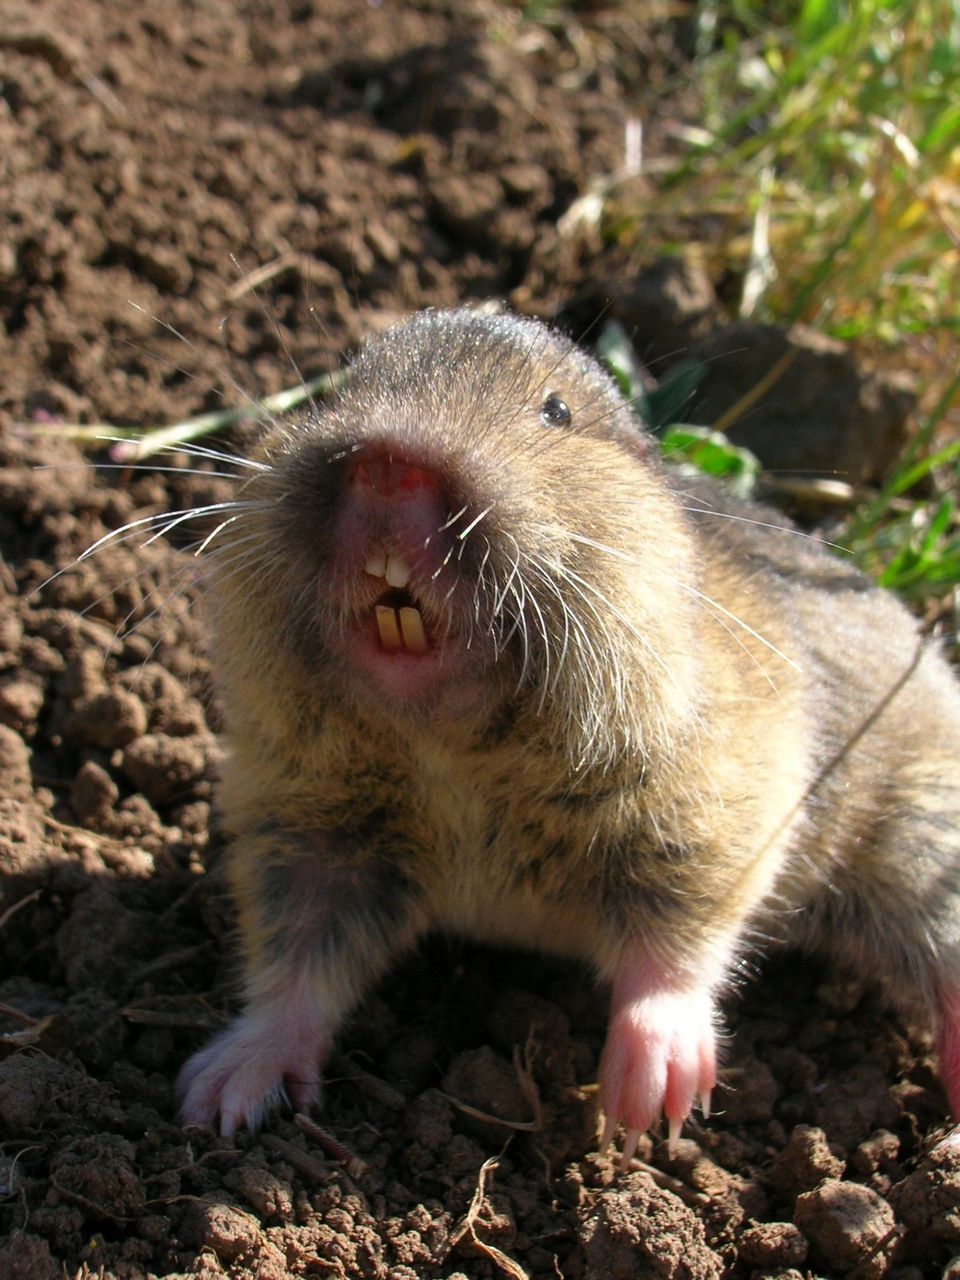
\includegraphics[width=0.3\textwidth]{figures/gophers/145893468_d8ad1675c0_o.jpg}\quad}
%\hfil
%\rlap{\quad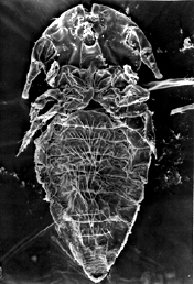
\includegraphics[width=0.3\textwidth]{figures/louse/thomomydoecus.png}}
\begin{pspicture}(18,12)
\psset{unit=0.3cm,linewidth=0.2,arrowsize=1}
\psline[linecolor=blue](0,0)(10,10)
\psline[linecolor=blue](4,0)(2,2)
\psline[linecolor=blue](8,0)(4,4)
\psline[linecolor=blue](12,0)(14,2)
\psline[linecolor=blue](16,0)(8,8)
\psline[linecolor=red](1,0)(11,10)
\psline[linecolor=red,arrows=-o](17,0)(9,8)
\psline[linecolor=red,arrows=-o](13,0)(15,2)
\psline[linecolor=red](7,3)(14,3)
\psline[linecolor=red,arrows=<-](10,3)(14,3)
\psline[linecolor=red](10,0)(7,3)
\psline[linecolor=red,arrows=-o](9,0)(5,4)
\psline[linecolor=red,arrows=-o](4,1)(3,2)
\rput{135}(4,1){\LARGE\textcolor{red}{\textsf{\textbf{x}}}}
\psline[linecolor=red](18,0)(17,1)
\psline[linecolor=red,arrows=*-](16,1)(17,1)
\end{pspicture}
}

\begin{document}

\frame{\titlepage}

\section{Introduction}

\begin{frame}{Symbiotic Interactions are Fundamental to Life}

\begin{columns}

\begin{column}{0.556\textwidth}
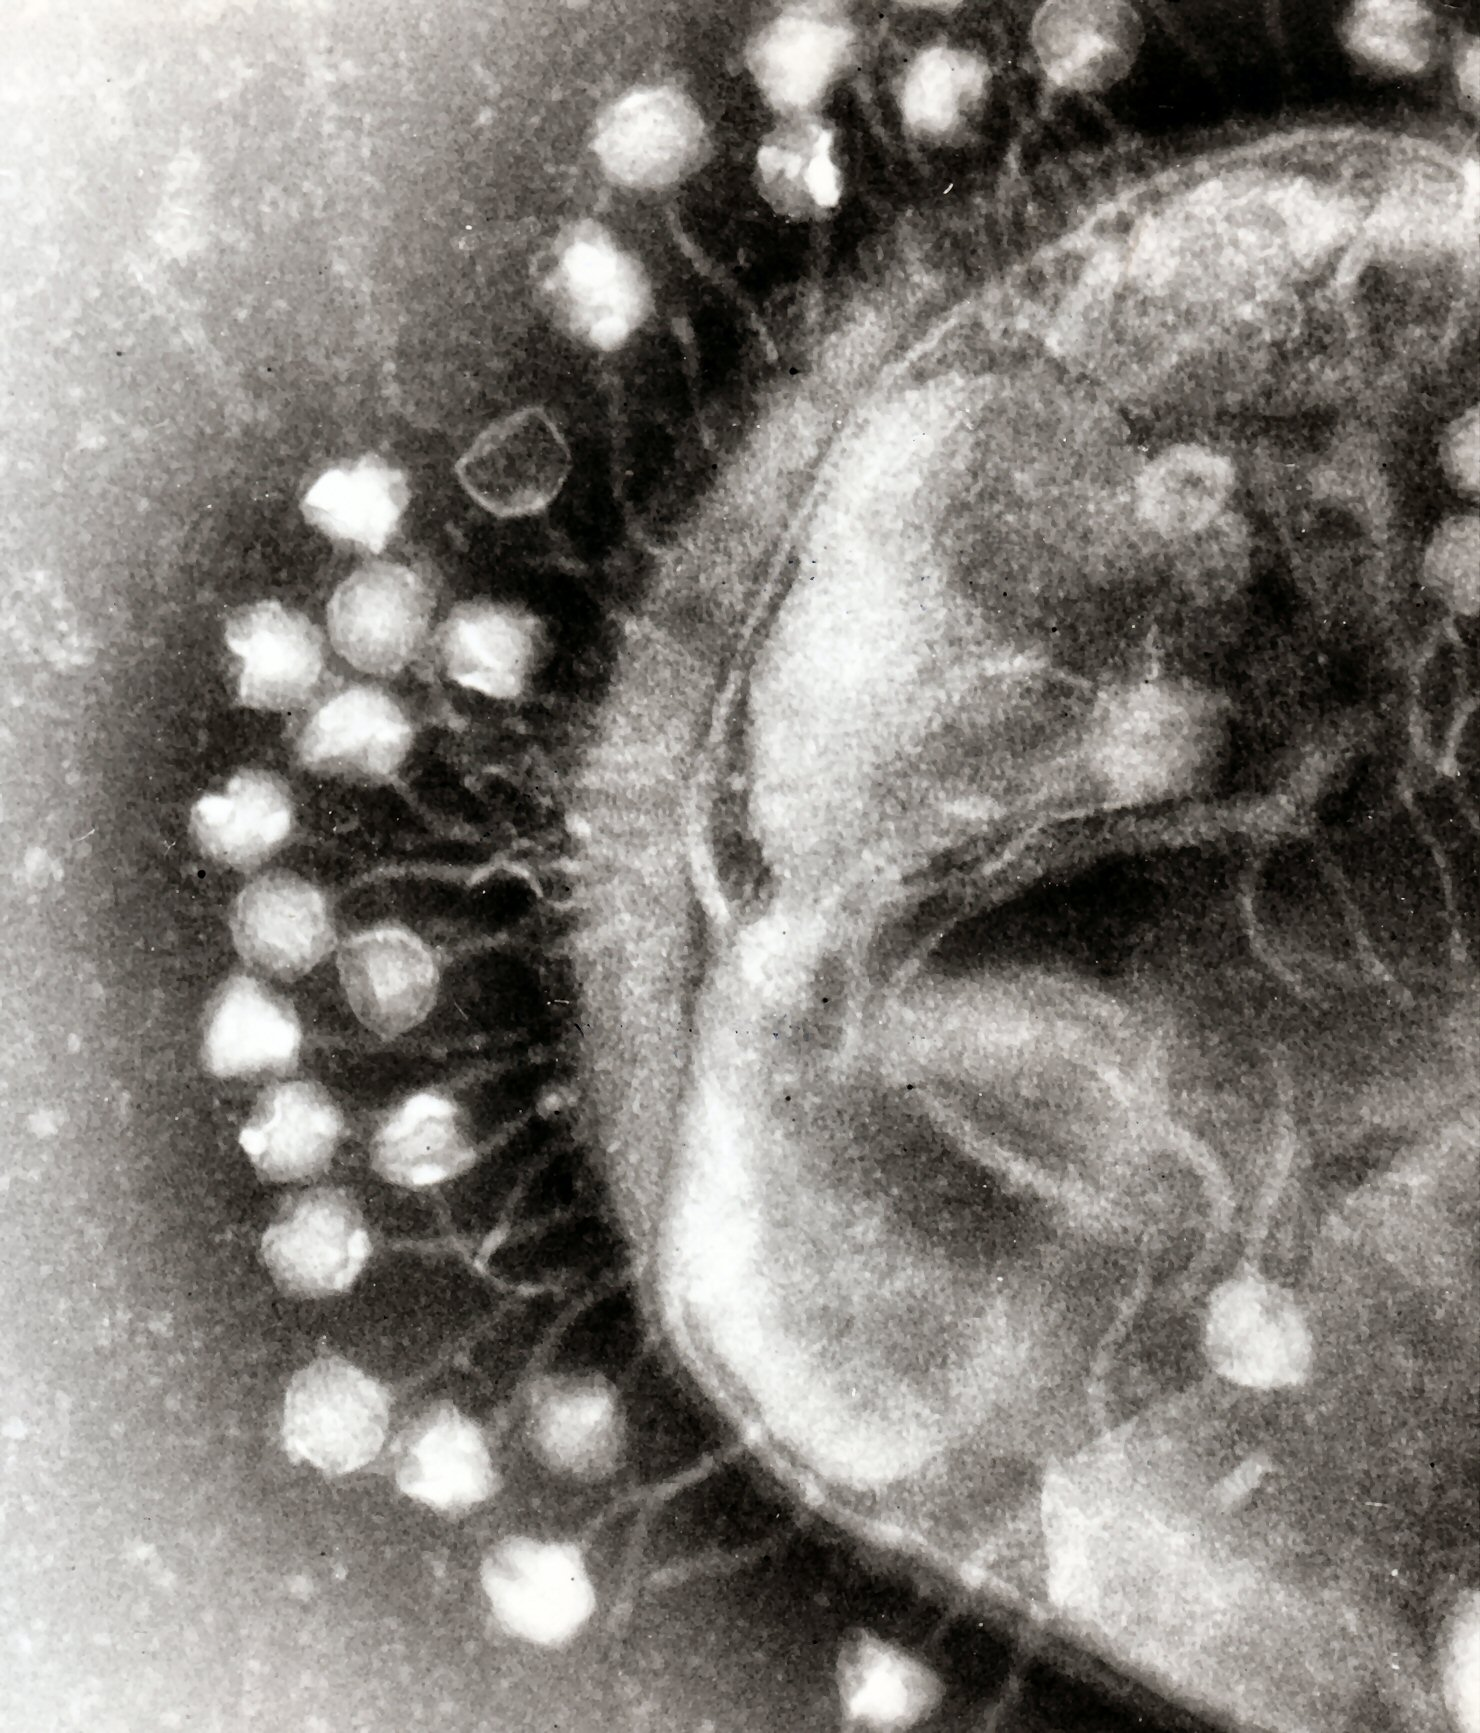
\includegraphics[width=\textwidth]{figures/symbioses/Phage.jpg}
\end{column}

\begin{column}{0.444\textwidth}
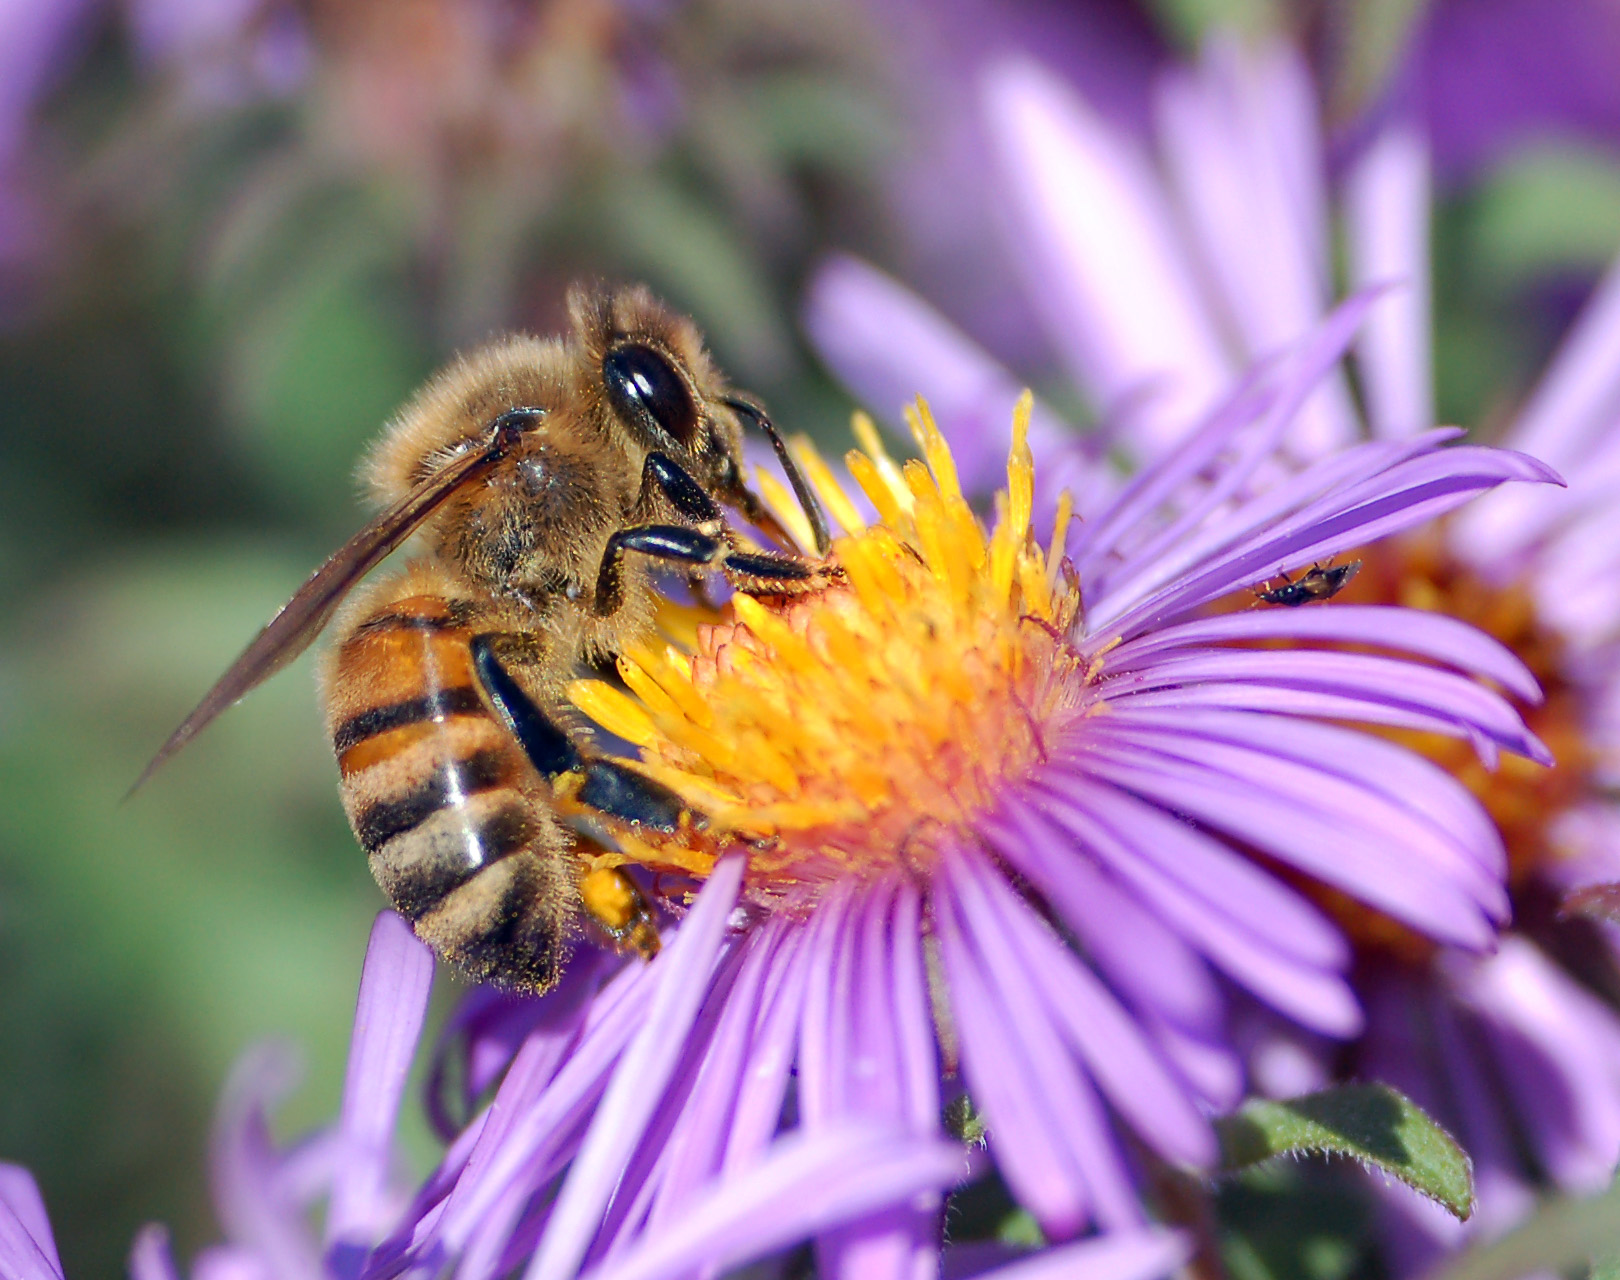
\includegraphics[width=\textwidth]{figures/symbioses/European_honey_bee_extracts_nectar.jpg}
\vfil
\includegraphics[width=\textwidth]{figures/symbioses/Clown_fish_in_the_Andaman_Coral_Reef.jpg}
\end{column}

\end{columns}

\end{frame}

\begin{frame}{Pocket Gophers and Chewing Lice}

\begin{columns}

\begin{column}{0.5\textwidth}
\centering
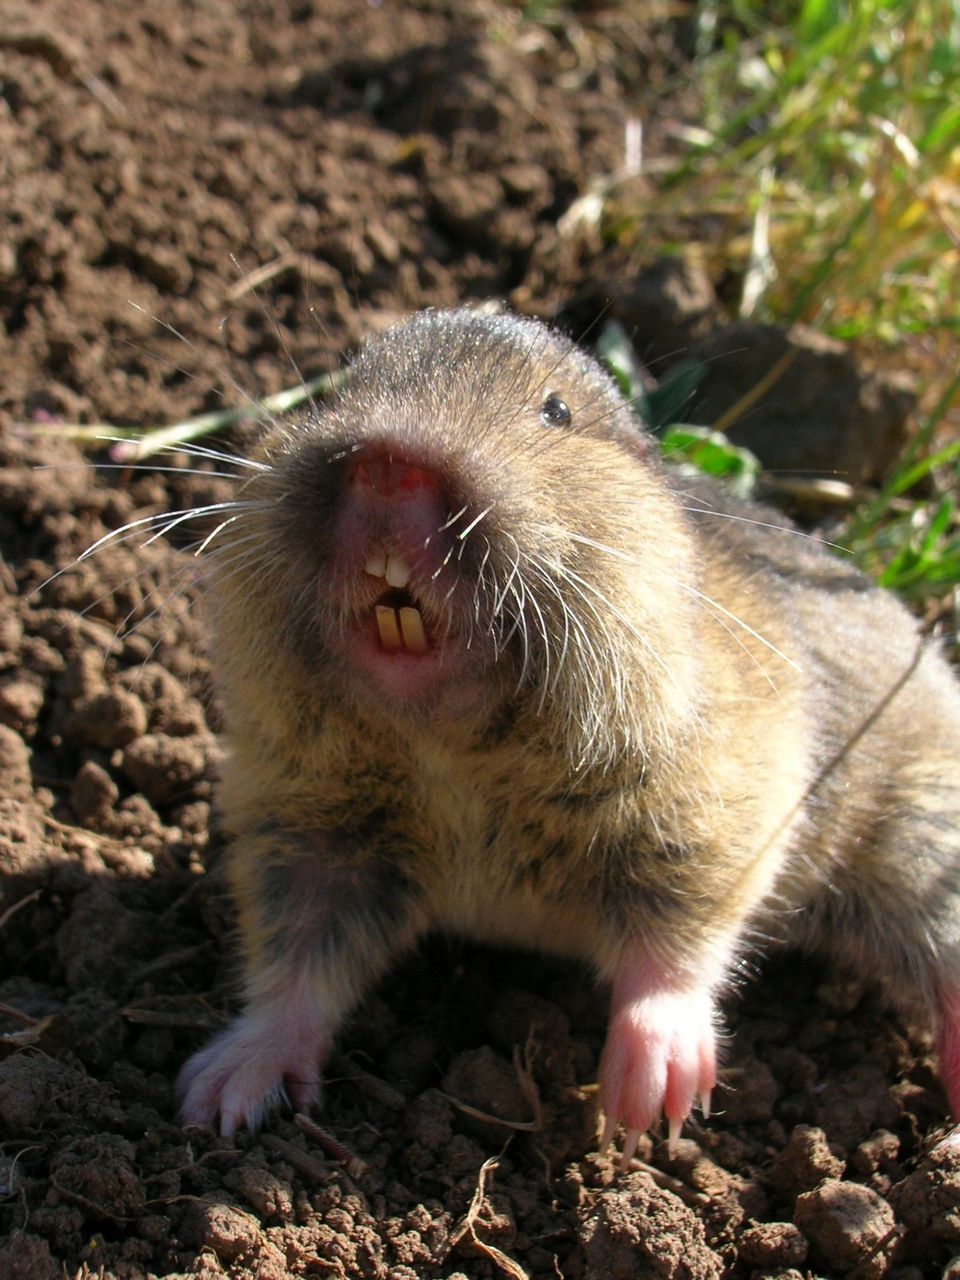
\includegraphics[height=2.5in]{figures/gophers/145893468_d8ad1675c0_o.jpg}

\emph{Thomomys bottae}\\\small Botta's Pocket Gopher
\end{column}

\begin{column}{0.5\textwidth}
\centering
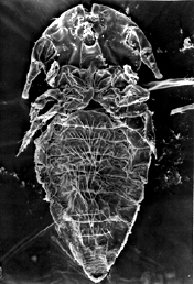
\includegraphics[height=2.5in]{figures/louse/thomomydoecus.png}

\emph{Thomomydoecus sp.}\\\small \hfil

\end{column}

\end{columns}

\end{frame}

\begin{frame}{Phylogenetic Trees are Evolutionary Models}

\begin{columns}

\only<2->{
\begin{column}{0.5\textwidth}
\centering
\begin{tikzpicture}
\node (gopherphy) {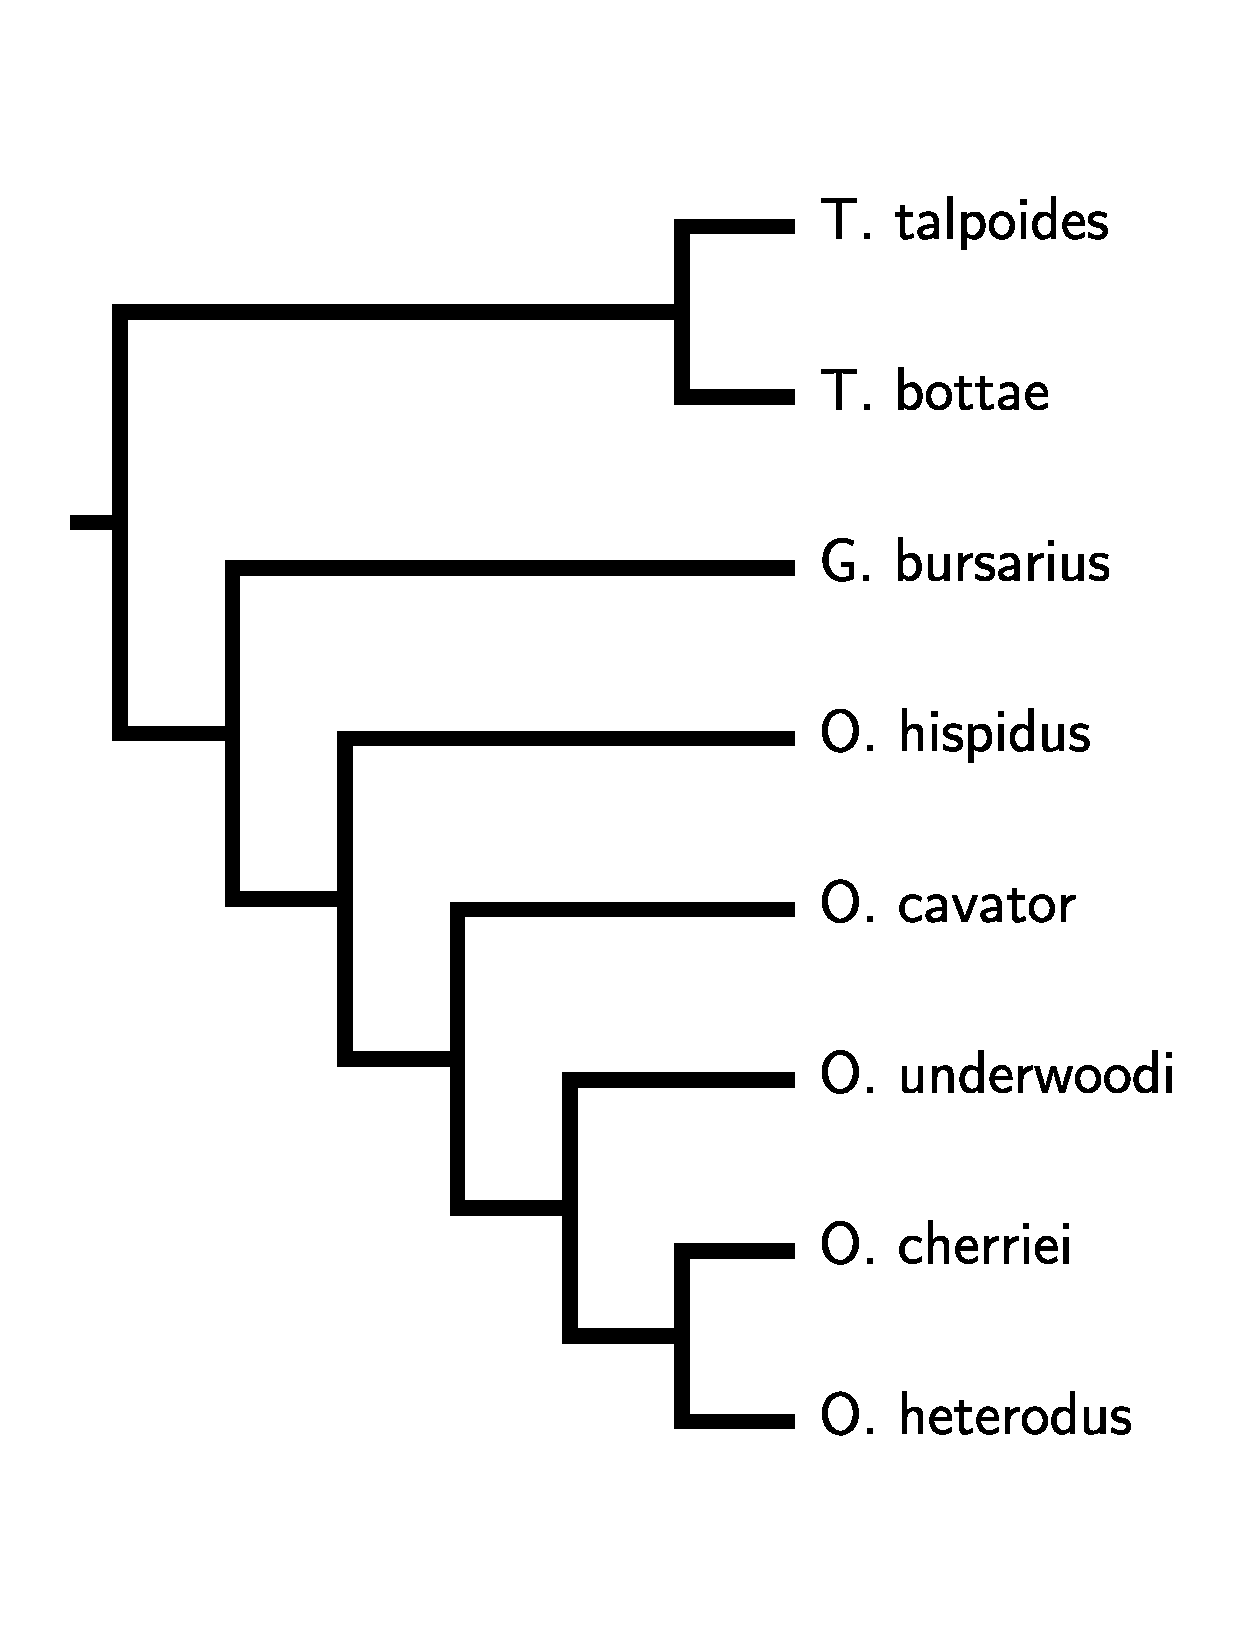
\includegraphics[height=2.5in]{figures/gopher.pdf}};
\node (gopher) at (-2, -2.5) {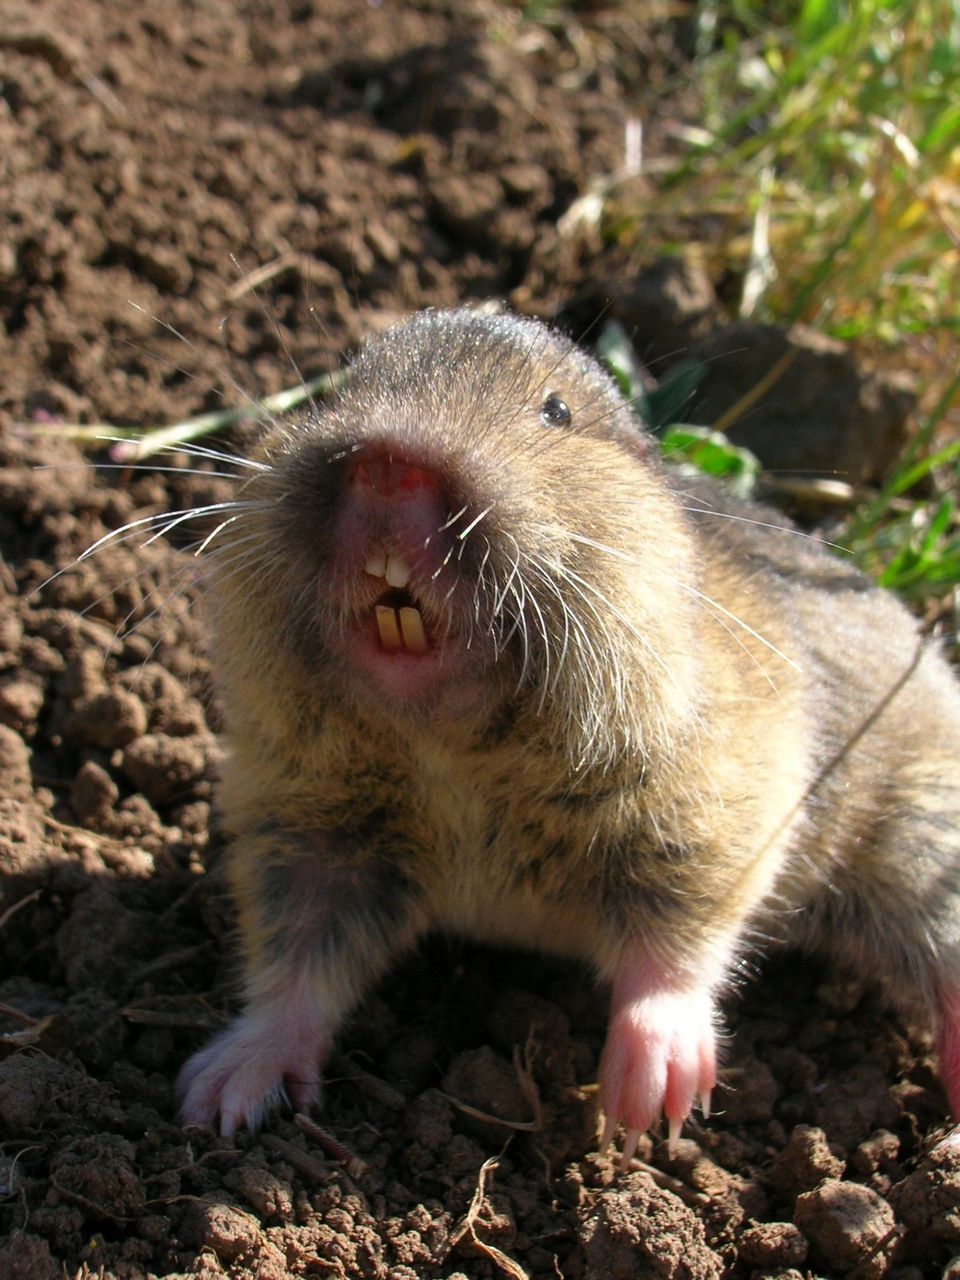
\includegraphics[width=0.6in]{figures/gophers/145893468_d8ad1675c0_o.jpg}};
\end{tikzpicture}
\end{column}
}

\only<2>{
\begin{column}{0.5\textwidth}
\end{column}
}

\only<3->{
\begin{column}{0.5\textwidth}
\centering
\begin{tikzpicture}
\node (lousephy) {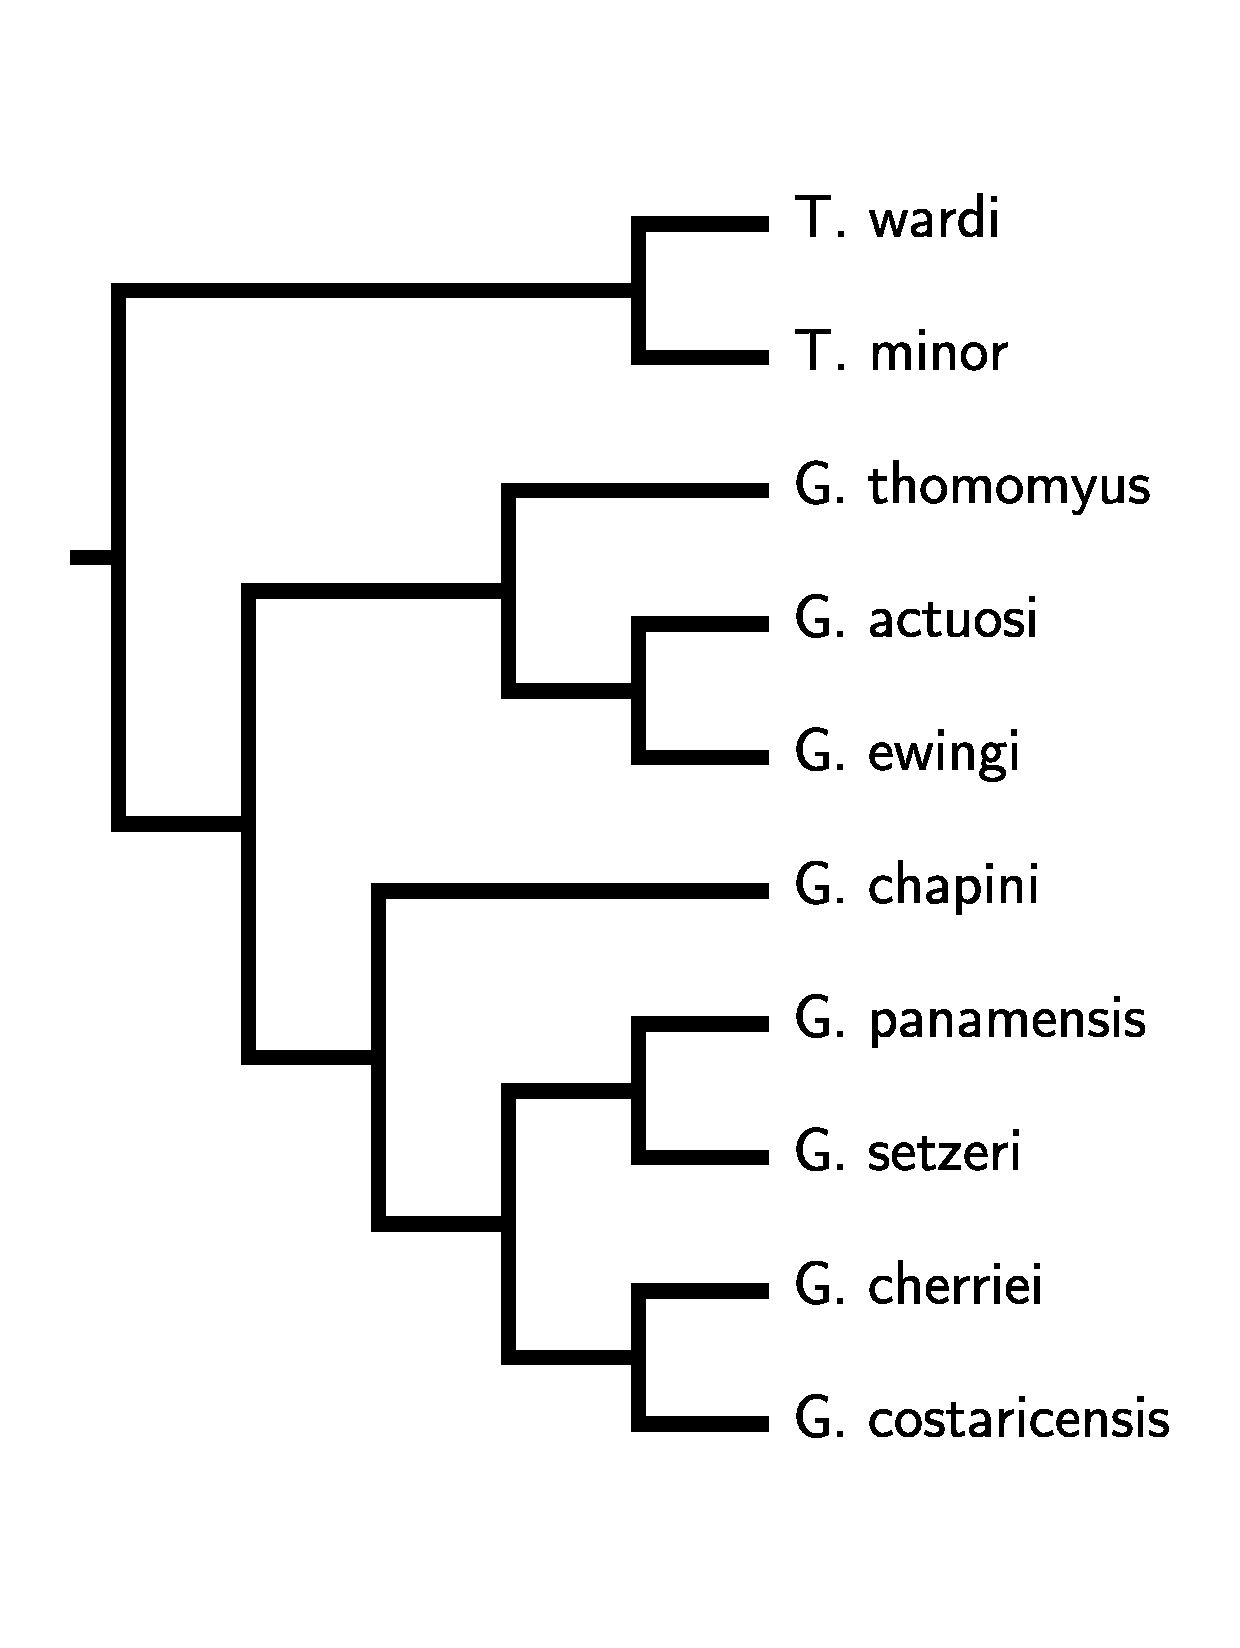
\includegraphics[height=2.5in]{figures/louse.pdf}};
\node (louse) at (-2.10, -2.5) {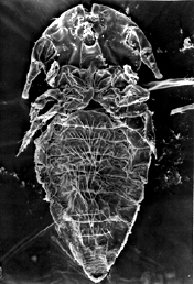
\includegraphics[width=0.6in]{figures/louse/thomomydoecus.png}};
\end{tikzpicture}
\end{column}
}

\end{columns}

\end{frame}

\begin{frame}{Coevolution is a Complex Process}
\centering
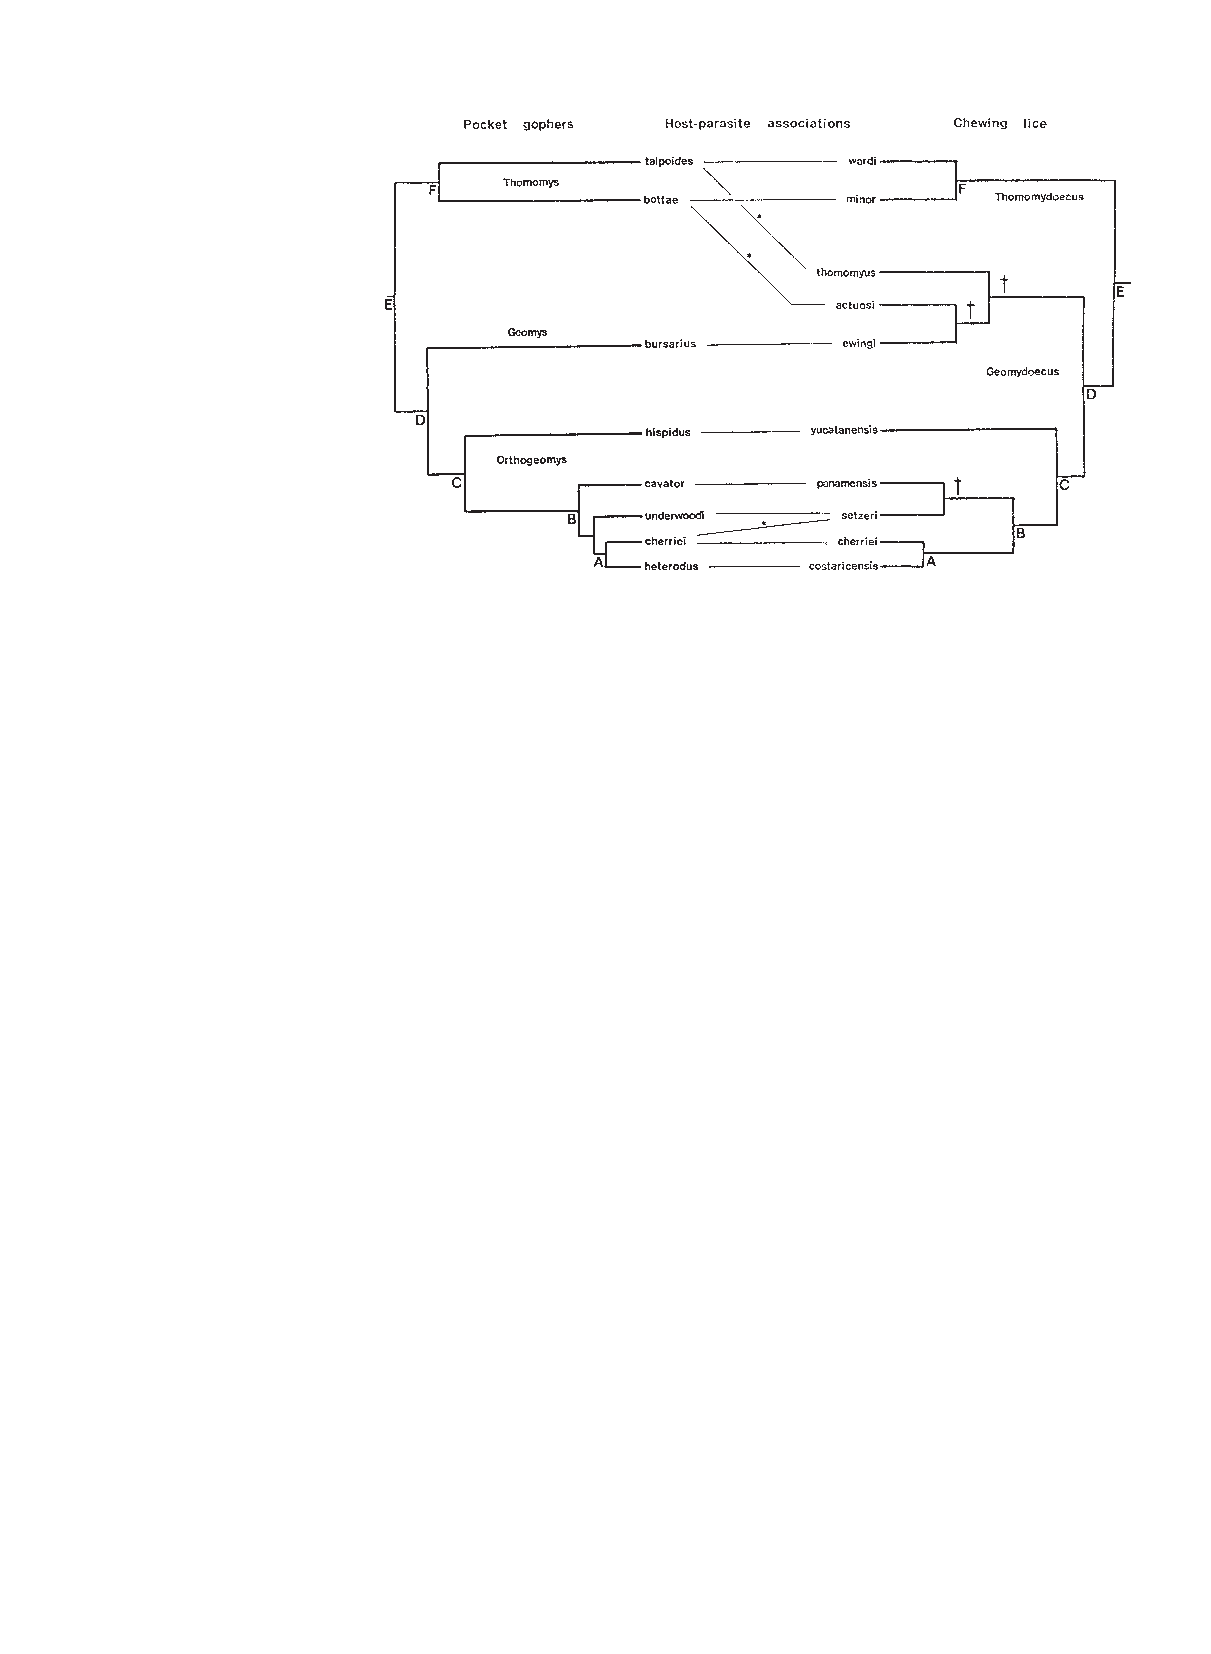
\includegraphics[width=\textwidth]{figures/gopher-louse.pdf}

\blfootnote{Hafner \& Nadler (1988), \emph{Nature 332}: 258--259}
\end{frame}

\begin{frame}{Coevolution is Event-Driven}
\vspace{-0.2in}
\centering
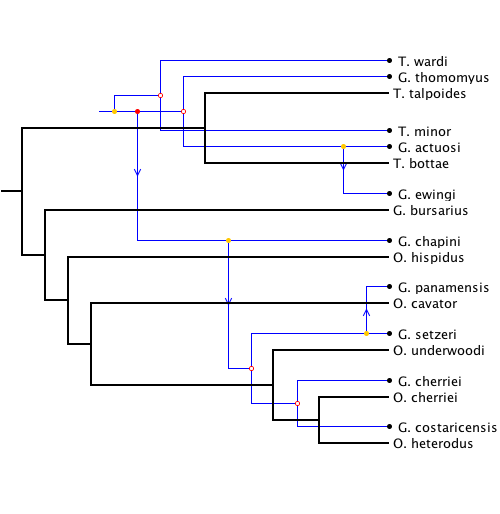
\includegraphics[width=0.8\textwidth]{figures/jane1.png}

\end{frame}

\begin{frame}{Reconstruction Methods Make Several Assumptions}
\vspace{-0.2in}
\centering
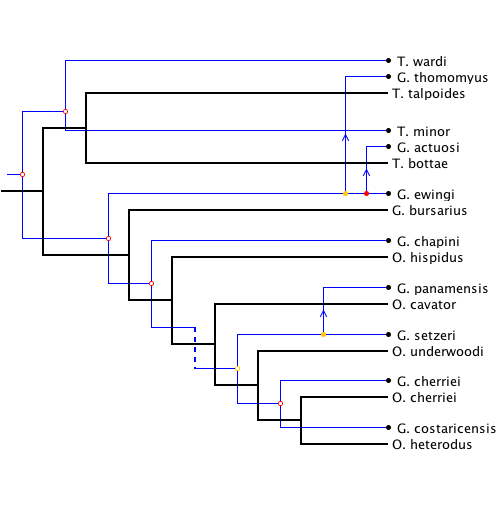
\includegraphics[width=0.8\textwidth]{figures/jane6.png}


\end{frame}

%\begin{frame}{Coevolutionary Events}
%
%\begin{columns}[c]
%
%\begin{column}{0.75\textwidth}
%
%\begin{pspicture}(18,12)
%\psset{unit=0.4cm,linewidth=0.2,arrowsize=1}
%\psline[linecolor=blue](0,0)(10,10)
%\psline[linecolor=blue](4,0)(2,2)
%\psline[linecolor=blue](8,0)(4,4)
%\psline[linecolor=blue](12,0)(14,2)
%\psline[linecolor=blue](16,0)(8,8)
%\psline[linecolor=red](1,0)(11,10)
%\psline[linecolor=red,arrows=-o](17,0)(9,8)
%\psline[linecolor=red,arrows=-o](13,0)(15,2)
%\psline[linecolor=red](7,3)(14,3)
%\psline[linecolor=red,arrows=<-](10,3)(14,3)
%\psline[linecolor=red](10,0)(7,3)
%\psline[linecolor=red,arrows=-o](9,0)(5,4)
%\psline[linecolor=red,arrows=-o](4,1)(3,2)
%\rput{135}(4,1){\LARGE\textcolor{red}{\textsf{\textbf{x}}}}
%\psline[linecolor=red](18,0)(17,1)
%\psline[linecolor=red,arrows=*-](16,1)(17,1)
%\end{pspicture}
%
%\end{column}
%
%\begin{column}{0.25\textwidth}
%
%Cospeciation
%
%\begin{pspicture}(1,1)
%\psline[linecolor=blue](0,0.5)(0.5,0.5)
%\psline[linecolor=blue](0.5,0.3)(1,0.3)
%\psline[linecolor=blue](0.5,0.7)(1,0.7)
%\psline[linecolor=blue](0.5,0.3)(0.5,0.7)
%\psline[linecolor=red](0.4,0.4)(1,0.4)
%\psline[linecolor=red](0.4,0.8)(1,0.8)
%\psline[linecolor=red](0.4,0.4)(0.4,0.8)
%\psline[linecolor=red,arrows=-o](0,0.6)(0.4,0.6)
%\end{pspicture}
%
%\vspace{0.25cm}
%
%Duplication
%
%\begin{pspicture}(1,1)
%\psline[linecolor=blue](0,0)(1,0)
%\psline[linecolor=red](0,0.1)(1,0.1)
%\psline[linecolor=red,arrows=*-](0.5,0.1)(0.5,0.3)
%\psline[linecolor=red](0.5,0.3)(1,0.3)
%\end{pspicture}
%
%\vspace{0.25cm}
%
%Host-Switch
%
%\begin{pspicture}(1,1)
%\psline[linecolor=blue](0,0)(1,0)
%\psline[linecolor=blue](0,0.4)(1,0.4)
%\psline[linecolor=red](0,0.1)(1,0.1)
%\psline[linecolor=red](0.5,0.1)(0.5,0.5)
%\psline[linecolor=red,arrows=->,arrowsize=0.1](0.5,0.1)(0.5,0.35)
%\psline[linecolor=red](0.5,0.5)(1,0.5)
%\end{pspicture}
%
%\vspace{0.25cm}
%
%Loss
%
%\begin{pspicture}(1,1)
%\psline[linecolor=blue](0,0)(1,0)
%\psline[linecolor=red](0,0.1)(0.8,0.1)
%\rput(0.8,0.1){\large\textcolor{red}{\textsf{\textbf{x}}}}
%\end{pspicture}
%
%\end{column}
%
%\end{columns}
%
%\end{frame}

\begin{frame}{Evolutionary Processes are Studied Probabilistically}

\centering

\begin{tikzpicture}
\draw[puzzle piece,thick] (0,4) to +(3,2);
\draw (1.5,5) node[align=center] {Molecular\\Evolution\\\small Felsenstein (1981)};
\draw[puzzle piece,thick] (3,4) to +(3,2);
\draw (4.5,5) node[align=center] {Population\\Genetics\\\small Kingman (1982)};
\draw[puzzle piece,thick] (6,4) to +(3,2);  
\draw (7.5,5) node[align=center] {Gene Evolution\\\small Arvestad et al.\\\small(2003)};                                                                      
\draw[puzzle piece,thick] (0,2) to +(3,2);
\draw (1.5,3) node[align=center] {Biogeography\\\small Lemey et al.\\\small(2009, 2010)};
\draw[puzzle piece,thick] (3,2) to +(3,2);
\draw (4.5,3) node[align=center] {Speciation\\\small Yang \& Rannala\\\small(2010)}; 
\onslide<2->{\draw (7.5,3) node[align=center] {Coevolution?};}  
% geography, gene-species trees, coalescent, clock models

\end{tikzpicture}


\end{frame}

\section{Methods}

\begin{frame}{A Bayesian Formulation for Coevolution}

\begin{equation*}
\overbrace{P\left(H,S,\R\mid D\right)}^{\mathclap{\text{probability of reconstruction}}} \onslide<2->{\propto \int_\theta \overbrace{P\left(d_H,d_S\mid H,S,\R,\theta\right)}^{\mathclap{\text{likelihood}}} \overbrace{P\left(H,S,\R,\theta\right)}^{\mathclap{\text{prior}}} \,\dif \theta}
\end{equation*}

\vspace{-12pt}

\onslide<3-4>{
\begin{block}{Likelihood}
\vspace{-12pt}
\begin{align*}
P\left(d_H,d_S\mid H,S,\R,\theta\right) &= P\left(d_H\mid H,S,\R,\theta\right)P\left(d_S\mid H,S,\R,\theta\right)\\
\onslide<4>{&= \underbrace{P\left(d_H\mid H\right)}_{\mathclap{\text{tree likelihood}}}\,\underbrace{P\left(d_S\mid S\right)}_{\mathclap{\text{tree likelihood}}}}
\end{align*}
\end{block}
}

\vspace{-96pt}

\onslide<5-6>{
\begin{block}{Prior}
\vspace{-12pt}
\begin{align*}
P\left(H,S,\R,\theta\right) &= P\left(S\mid H,\R,\theta\right)P\left(H,\R,\theta\right)\\
\onslide<6>{&= \underbrace{P\left(S\mid H,\R,\theta\right)}_{\mathclap{\text{?}}}\underbrace{P\left(H\right)P\left(\R\right)P\left(\theta\right)}_{\mathclap{\text{existing/trivial priors}}}}
\end{align*}
\end{block}
}

\vfill

$H = \text{host tree}, S = \text{symbiont tree}, \R = \text{reconciliation},$\\$\theta = \text{coevolutionary rates}, D, d_H, d_S = \text{sequence data}$

\end{frame}

\begin{frame}{Approximating the Symbiont Tree Prior, $P\left(S\mid H,\R,\theta\right)$}

\begin{itemize}

\item Cannot be calculated easily because of infinite permutations of unobserved events \pause
\item Approximation by considering only observed events \pause
\item Observation of duplication, host-switch, and loss events are modeled as independent Poisson processes \pause
\item Cospeciation assumed to occur whenever host speciates \pause
\item Algorithm identifies between 7~cases to calculate probability of observation \pause
\item Any uncertainties are integrated out

\end{itemize}

\end{frame}

\begin{frame}{The Cases}
\centering
\hspace{-2.15em}
\begin{tabular}{c c c c}

\psset{unit=1.0in,linewidth=0.02}

\begin{pspicture}(1,1)
\psline[linecolor=blue](0,0)(1,0)
\psline[linecolor=red](0,0.1)(1,0.1)
\psline[linecolor=red,arrows=*-](0.5,0.1)(0.5,0.2)
\psline[linecolor=red](0.5,0.2)(1,0.2)
\end{pspicture}

&
\begin{pspicture}(1,1)
\psline[linecolor=blue](0,0)(1,0)
\psline[linecolor=blue](0,0.4)(1,0.4)
\psline[linecolor=red](0,0.1)(1,0.1)
\psline[linecolor=red](0.5,0.1)(0.5,0.5)
\psline[linecolor=red,arrows=->,arrowsize=0.1](0.5,0.1)(0.5,0.35)
\psline[linecolor=red](0.5,0.5)(1,0.5)
\psline[linecolor=blue,linestyle=dashed](0.7,0.4)(0.7,0.25)
\psline[linecolor=blue,linestyle=dashed](0.7,0.25)(1,0.25)
\end{pspicture}
&
\begin{pspicture}(1,1)
\psline[linecolor=blue](0,0)(1,0)
\psline[linecolor=blue](0,0.4)(1,0.4)
\psline[linecolor=red](0,0.1)(1,0.1)
\psline[linecolor=red](0.5,0.1)(0.5,0.5)
\psline[linecolor=red,arrows=->,arrowsize=0.1](0.5,0.1)(0.5,0.35)
\psline[linecolor=red](0.5,0.5)(1,0.5)
\psline[linecolor=blue,linestyle=dashed](0.7,0.4)(0.7,0.25)
\psline[linecolor=blue,linestyle=dashed](0.7,0.25)(1,0.25)
\psline[linecolor=blue,linestyle=dashed](0.6,0.0)(0.6,-0.3)
\psline[linecolor=blue,linestyle=dashed](0.6,-0.3)(1,-0.3)
\psline[linecolor=blue,linestyle=dashed](0.8,0.0)(0.8,-0.15)
\psline[linecolor=blue,linestyle=dashed](0.8,-0.15)(1,-0.15)
\end{pspicture}
\\
\begin{pspicture}(1,1)
\psline[linecolor=blue](0,0.5)(0.5,0.5)
\psline[linecolor=blue](0.5,0.3)(1,0.3)
\psline[linecolor=blue](0.5,0.7)(1,0.7)
\psline[linecolor=blue](0.5,0.3)(0.5,0.7)
\psline[linecolor=red](0.4,0.4)(1,0.4)
\psline[linecolor=red](0.4,0.8)(1,0.8)
\psline[linecolor=red](0.4,0.4)(0.4,0.8)
\psline[linecolor=red,arrows=-o](0,0.6)(0.4,0.6)
\psline[linecolor=blue,linestyle=dashed](0.6,0.3)(0.6,0.0)
\psline[linecolor=blue,linestyle=dashed](0.6,0.0)(1,0.0)
\psline[linecolor=blue,linestyle=dashed](0.8,0.3)(0.8,0.15)
\psline[linecolor=blue,linestyle=dashed](0.8,0.15)(1,0.15)
\psline[linecolor=blue,linestyle=dashed](0.7,0.7)(0.7,0.55)
\psline[linecolor=blue,linestyle=dashed](0.7,0.55)(1,0.55)
\end{pspicture}
&
\begin{pspicture}(1,1)
\psline[linecolor=blue](0,0.5)(0.5,0.5)
\psline[linecolor=blue](0.5,0.3)(1,0.3)
\psline[linecolor=blue](0.5,0.7)(1,0.7)
\psline[linecolor=blue](0.5,0.3)(0.5,0.7)
\psline[linecolor=red](0.4,0.4)(1,0.4)
\psline[linecolor=red](0.4,0.8)(0.8,0.8)
\rput(0.8,0.8){\textcolor{red}{\LARGE\textsf{x}}}
\psline[linecolor=red](0.65,0.8)(0.65,0.5)
\psline[linecolor=red,arrows=->,arrowsize=0.1](0.65,0.8)(0.65,0.55)
\psline[linecolor=red](0.65,0.5)(1,0.5)
\psline[linecolor=red](0.4,0.4)(0.4,0.8)
\psline[linecolor=red,arrows=-o](0,0.6)(0.4,0.6)
\psline[linecolor=blue,linestyle=dashed](0.6,0.3)(0.6,0.0)
\psline[linecolor=blue,linestyle=dashed](0.6,0.0)(1,0.0)
\psline[linecolor=blue,linestyle=dashed](0.8,0.3)(0.8,0.15)
\psline[linecolor=blue,linestyle=dashed](0.8,0.15)(1,0.15)
\end{pspicture}
&
\begin{pspicture}(1,1)
\psline[linecolor=blue](0,0.5)(0.5,0.5)
\psline[linecolor=blue](0.5,0.3)(1,0.3)
\psline[linecolor=blue](0.5,0.7)(1,0.7)
\psline[linecolor=blue](0.5,0.3)(0.5,0.7)
\psline[linecolor=red](0.4,0.4)(1,0.4)
\psline[linecolor=red](0.4,0.8)(0.9,0.8)
\psline[linecolor=red](0.4,0.4)(0.4,0.8)
\psline[linecolor=red,arrows=-o](0,0.6)(0.4,0.6)
\psline[linecolor=red](0.3,0.46)(1.0,0.46)
\psline[linecolor=red](0.3,0.9)(0.7,0.9)
\psline[linecolor=red](0.3,0.46)(0.3,0.9)
\psline[linecolor=red,arrows=-o](0.15,0.7)(0.3,0.7)
\psline[linecolor=red,arrows=*-](0.15,0.6)(0.15,0.7)
\psline[linecolor=blue,linestyle=dashed](0.6,0.3)(0.6,0.0)
\psline[linecolor=blue,linestyle=dashed](0.6,0.0)(1,0.0)
\psline[linecolor=blue,linestyle=dashed](0.8,0.3)(0.8,0.15)
\psline[linecolor=blue,linestyle=dashed](0.8,0.15)(1,0.15)
\rput(0.7,0.9){\textcolor{red}{\LARGE\textsf{x}}}
\rput(0.9,0.8){\textcolor{red}{\LARGE\textsf{x}}}
\end{pspicture}
&
\begin{pspicture}(1,1)
\psline[linecolor=blue](0,0)(1,0)
\psline[linecolor=blue](0,0.4)(1,0.4)
\psline[linecolor=blue](0,0.8)(1,0.8)
\psline[linecolor=red](0,0.5)(0.85,0.5)
\rput(0.85,0.5){\textcolor{red}{\LARGE\textsf{x}}}
\psline[linecolor=red](0.6,0.5)(0.6,0.9)
\psline[linecolor=red,arrows=->,arrowsize=0.1](0.6,0.5)(0.6,0.75)
\psline[linecolor=red](0.6,0.9)(1,0.9)
\psline[linecolor=red](0.3,0.5)(0.3,0.1)
\psline[linecolor=red,arrows=->,arrowsize=0.1](0.3,0.5)(0.3,0.2)
\psline[linecolor=red](0.3,0.1)(1,0.1)
\psline[linecolor=blue,linestyle=dashed](0.7,0.8)(0.7,0.65)
\psline[linecolor=blue,linestyle=dashed](0.7,0.65)(1,0.65)
\psline[linecolor=blue,linestyle=dashed](0.6,0.0)(0.6,-0.3)
\psline[linecolor=blue,linestyle=dashed](0.6,-0.3)(1,-0.3)
\psline[linecolor=blue,linestyle=dashed](0.8,0.0)(0.8,-0.15)
\psline[linecolor=blue,linestyle=dashed](0.8,-0.15)(1,-0.15)
\end{pspicture}
\end{tabular}
\vfill
\textcolor{blue}{\textbf{Host}} / \textcolor{red}{\textbf{Symbiont}}

%\begin{itemize}
%\item Events are modeled as independent Poisson processes\\
%\item Duplication rate $\lambda$, host-switch rate $\tau$, and loss rate $\mu$,
%with overall event rate $\Lambda = \lambda + \tau + \mu$
%\item Cospeciation events assumed to occur whenever host speciates
%\end{itemize}
%
%\begin{block}{Duplication Events}
%
%\begin{equation}
%P_D\left(t\right) = \lambda e ^ {-\Lambda t}
%\end{equation}
%
%\end{block}
%
%\begin{block}{Host-Switch Events}
%\begin{equation}
%P_{HS}\left(t\right) = \frac{\tau e ^ {-\Lambda t}}{n-1}
%\end{equation}
%where $n$ is the number of host lineages contemporaneous with the symbiont
%
%\end{block}

\end{frame}

\begin{frame}{An Example Case}
\centering
\begin{pspicture}(1,1)
\psset{unit=2in, linewidth=0.02}
\uncover<2->{\psline[linestyle=dotted,arrows=-](-0.3,-0.3)(1.7,-0.3)}
\psline[linecolor=blue](0.0,-0.0)(0.0,-1.0)
\psline[linecolor=blue](0.4,-0.0)(0.4,-1.0)
\psline[linecolor=blue](0.8,-0.0)(0.8,-1.0)
\psline[linecolor=red](0.5,-0.0)(0.5,-0.85)
\rput{90}(0.5,-0.85){\textcolor{red}{\Huge\textsf{x}}}
\visible<1-2>{
\psline[linecolor=red](0.5,-0.4)(0.9,-0.4)
\psline[linecolor=red,arrows=->,arrowsize=0.1](0.5,-0.4)(0.75,-0.4)
\psline[linecolor=red](0.9,-0.4)(0.9,-1.0)
}
\visible<3>{
\psline[linecolor=red](0.5,-0.5)(0.9,-0.5)
\psline[linecolor=red,arrows=->,arrowsize=0.1](0.5,-0.5)(0.75,-0.5)
\psline[linecolor=red](0.9,-0.5)(0.9,-1.0)
}
\visible<4-5>{
\psline[linecolor=red](0.5,-0.6)(0.9,-0.6)
\psline[linecolor=red,arrows=->,arrowsize=0.1](0.5,-0.6)(0.75,-0.6)
\psline[linecolor=red](0.9,-0.6)(0.9,-1.0)
}
\psline[linecolor=red](0.5,-0.3)(0.1,-0.3)
\psline[linecolor=red,arrows=->,arrowsize=0.1](0.5,-0.3)(0.2,-0.3)
\psline[linecolor=red](0.1,-0.3)(0.1,-1.0)
\psline[linecolor=blue,linestyle=dashed](0.8,-0.7)(0.65,-0.7)
\psline[linecolor=blue,linestyle=dashed](0.65,-0.7)(0.65,-1.0)
\psline[linecolor=blue,linestyle=dashed](0.0,-0.6)(-0.3,-0.6)
\psline[linecolor=blue,linestyle=dashed](-0.3,-0.6)(-0.3,-1.0)
\psline[linecolor=blue,linestyle=dashed](0.0,-0.8)(-0.15,-0.8)
\psline[linecolor=blue,linestyle=dashed](-0.15,-0.8)(-0.15,-1.0)
\uncover<5->{
\psline[linecolor=blue](0.8,-0.7)(0.65,-0.7)
\psline[linecolor=blue](0.65,-0.7)(0.65,-1.0)
}
\visible<5>{
\psline[linecolor=red](0.7,-0.75)(0.9,-0.75)
\psline[linecolor=red](0.7,-0.75)(0.7,-0.9)
\rput{90}(0.7,-0.9){\textcolor{red}{\Huge\textsf{x}}}
}
\visible<6->{
\psline[linecolor=red](0.5,-0.8)(0.9,-0.8)
\psline[linecolor=red,arrows=->,arrowsize=0.1](0.5,-0.8)(0.75,-0.8)
\psline[linecolor=red](0.9,-0.8)(0.9,-1.0)
}
% 2nd tree
\visible<2->{
\psline(1.5,0)(1.5,-0.3)
\psline(1.3,-0.3)(1.7,-0.3)
\psline(1.3,-0.3)(1.3,-1)
\psline(1.7,-0.3)(1.7,-1)
}
\psline[strokeopacity=0,arrows=-](1.7,-0.3)(1.7,-1)
\end{pspicture}
\vfill
\textcolor{blue}{\textbf{Host}} / \textcolor{red}{\textbf{Symbiont}}

\pause\pause\pause\pause\pause

%\begin{block}{Loss Events}
%
%\begin{equation}
%P_{L}(t) = \int_0^t \mu e^{-\Lambda x} \, \dif x = \frac{\mu - \mu e ^ {-\Lambda t}}{\Lambda}
%\end{equation}
%
%\begin{equation}
%P_{\emptyset}\left(t\right) = e ^ {-\Lambda t}
%\end{equation}
%
%\vspace{18pt}
%
%\begin{columns}[c]
%
%\begin{column}{0.33\textwidth}
%\centering
%\begin{pspicture}(18,12)
%\psset{unit=0.3cm,linewidth=0.2}
%\psline[linecolor=blue](-1,0)(5,6)
%\psline[linecolor=blue](3,0)(1,2)
%\psline[linecolor=blue](7,0)(3,4)
%\psline[linecolor=red](4,4)(6,6)
%\rput{45}(4,4){\LARGE\textcolor{red}{\textsf{\textbf{x}}}}
%\end{pspicture}
%\end{column}
%
%\begin{column}{0.33\textwidth}
%\centering
%\begin{pspicture}(18,12)
%\psset{unit=0.3cm,linewidth=0.2}
%\psline[linecolor=blue](-1,0)(5,6)
%\psline[linecolor=blue](3,0)(1,2)
%\psline[linecolor=blue](7,0)(3,4)
%\psline[linecolor=red](2,2)(6,6)
%\psline[linecolor=red](8,0)(4,4)
%\rput{45}(2,2){\LARGE\textcolor{red}{\textsf{\textbf{x}}}}
%\rput{135}(8,0){\LARGE\textcolor{red}{\textsf{\textbf{x}}}}
%\end{pspicture}
%\end{column}
%
%\begin{column}{0.33\textwidth}
%\centering
%\begin{pspicture}(18,12)
%\psset{unit=0.3cm,linewidth=0.2}
%\psline[linecolor=blue](-1,0)(5,6)
%\psline[linecolor=blue](3,0)(1,2)
%\psline[linecolor=blue](7,0)(3,4)
%\psline[linecolor=red](0,0)(6,6)
%\psline[linecolor=red](4,0)(2,2)
%\psline[linecolor=red](8,0)(4,4)
%\rput{45}(0,0){\LARGE\textcolor{red}{\textsf{\textbf{x}}}}
%\rput{135}(4,0){\LARGE\textcolor{red}{\textsf{\textbf{x}}}}
%\rput{135}(8,0){\LARGE\textcolor{red}{\textsf{\textbf{x}}}}
%\end{pspicture}
%\end{column}
%
%\end{columns}
%
%\end{block}

\end{frame}

\begin{frame}{Bayesian MCMC Implementation}

\begin{itemize}

\item Probability of a reconstruction cannot be determined analytically \pause
\item Approximated using Markov chain Monte Carlo (MCMC)
\begin{itemize}
\item MCMC uses a random walk to explore the parameter-space
\end{itemize}
\pause
\item Algorithm implemented as a Java plug-in for BEAST, an existing program for evolutionary analysis via Bayesian MCMC \pause
\item All parameters estimated simultaneously
\begin{itemize}
\item host tree
\item symbiont tree
\item reconciliation
\end{itemize}

\end{itemize}

\end{frame}

\section{Simulation Results}

\begin{frame}{Simulation Results}

%\begin{itemize}
%\item 8 host taxa and 8 symbiont taxa with perfectly matching trees
%\end{itemize}

\centering

\begin{tabular}{r | r r | r r}
\multicolumn{1}{c}{} & \multicolumn{2}{c}{\textsc{simulation 1}} & \multicolumn{2}{c}{\textsc{simulation 2}} \\
\textbf{Rate} & \textbf{Actual} & \textbf{Estimated} & \textbf{Actual} & \textbf{Estimated} \\
\hline
duplication & 0.0 & $6.418 \times 10^{-2}$ & 1.0 & 1.419 \\
host-switch & 0.0 & $6.295 \times 10^{-2}$ & 1.0 & 2.471 \\
loss & 0.0 & $5.416 \times 10^{-2}$ & 1.0 & 1.606\\
\end{tabular}

\pause

\begin{columns}

\begin{column}{0.5\textwidth}
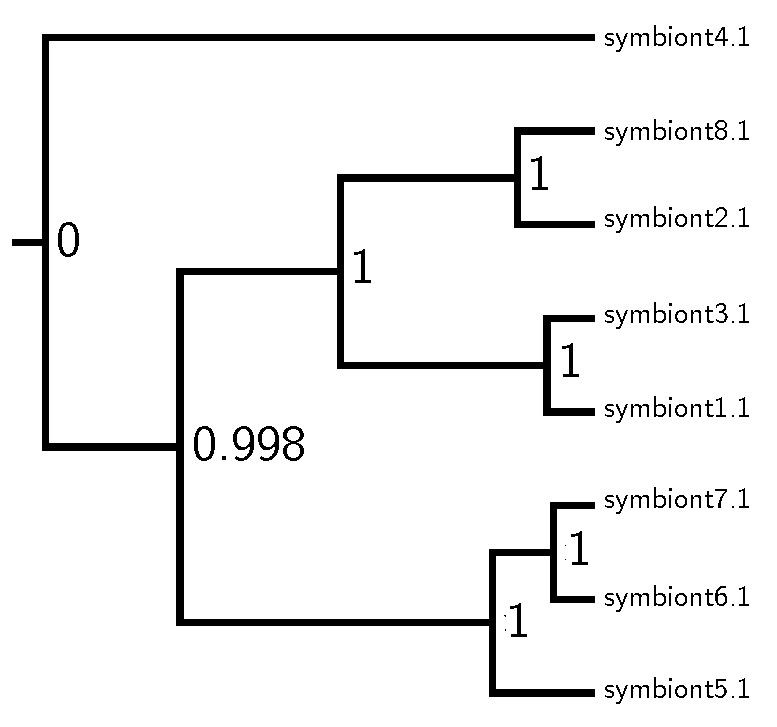
\includegraphics[width=\textwidth]{figures/sim1.pdf}
\end{column}

\begin{column}{0.5\textwidth}
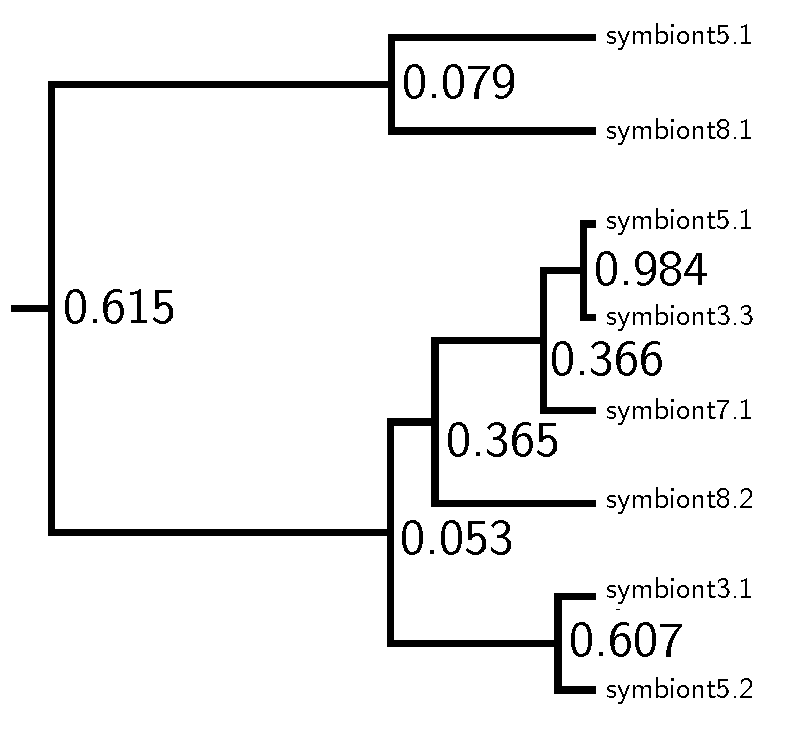
\includegraphics[width=\textwidth]{figures/sim2.pdf}
\end{column}

\end{columns}
\end{frame}

\section{Closing Remarks}

\begin{frame}{Contributions}

\begin{itemize}
\item Formulated an expression for the probability of a coevolutionary reconstruction \pause
\item Developed an algorithm to approximate the probability of symbiont tree for a reconstruction \pause
\item Implemented the algorithm in a popular, widely-used phylogenetics program
\end{itemize}

\end{frame}

\begin{frame}{Future Work}

\begin{itemize}
\item Analysis of real datasets \pause
\item Model for preferential host-switching \pause
\item Integration with other evolutionary models\\(e.g., biogeography) \pause
\item Hypothesis-testing of coevolutionary theories

\end{itemize}

\end{frame}

\begin{frame}{Acknowledgements}

\begin{itemize}

\item My mentors, Dr.~Yi-Chieh~Jessica~Wu, Rachel~Sealfon, and Prof.~Mukul~Bansal

\item Andrew~Brownjohn, Jon~Sanders, Prof.~Ran~Libeskind-Hadas, Hayden~Metsky, and Prof.~Manolis~Kellis, for their support

\item Dr.~Susan~Offner, for inspiring me

\item My family

\item Siemens Foundation and College Board

\item George Washington University

\end{itemize}

\end{frame}

\oldsection{}

\begin{frame}{References}
\small
\begin{hangparas}{2em}{1}
Baum, D. A. \& Offner, S. (2008). \emph{The American Biology Teacher, 70}(4), 222--229.

Bayes, T. \& Price, R. (1763). \emph{Phil. Trans. 53}, 370--418.

Charleston, M. A. (2009). A new likelihood method for cophylogenetic analysis.

Drummond, A. J., et al. (2012). \emph{Mol. Biol. Evol. 29}(8), 1969--1973.

Faria, N. R., et al. (2013). \emph{Phil. Trans. R. Soc. B, 368}(1614).

Felsenstein, J. (1981). \emph{J. Mol. Evol. 17}(6), 368--376.

Felsenstein, J. (2004). \emph{Inferring phylogenies}. Sunderland, MA: Sinauer.

Hafner, M. S. \& Nadler, S. A. (1988). \emph{Nature, 332}(6161), 258--259.

Huelsenbeck, J. P., Rannala, B., \& Larget, B. (2000). \emph{Evolution, 54}(2), 352--364.

Kingman, J. F. C. (1982). \emph{Stochastic Processes and their Applications, 13}(3), 235--248.

Segraves, K. A. (2010). \emph{Evo. Edu. Outreach, 3}(1), 62--70.

Sj\"ostrand, J., et al. (In prep.). A Bayesian method for analyzing lateral gene transfer.
\end{hangparas}
\end{frame}

\end{document}